\documentclass[border=8pt]{standalone}
\usepackage{tikz}
\usetikzlibrary{positioning,arrows.meta,shapes.misc,fit,backgrounds}

\begin{document}
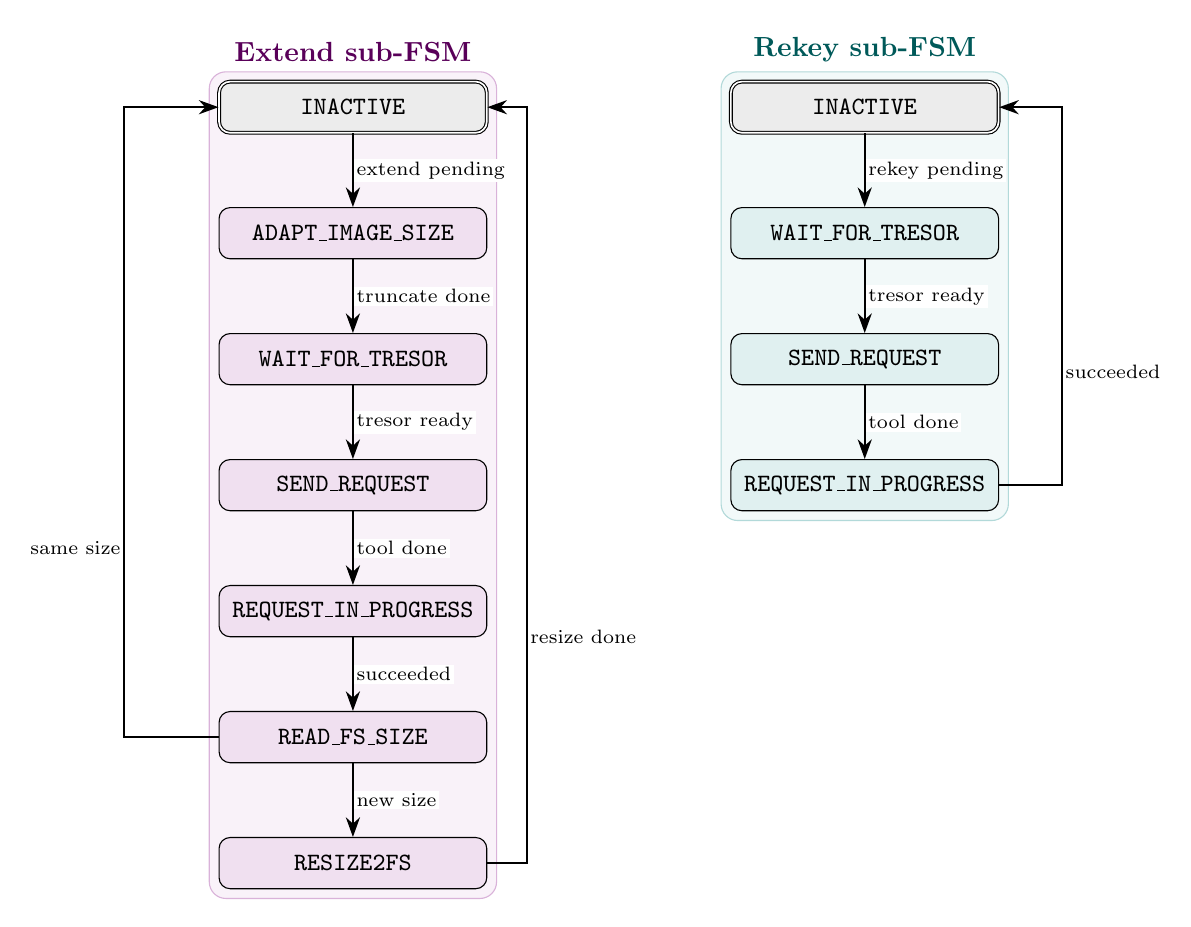
\begin{tikzpicture}[
  st/.style={draw, rectangle, rounded corners=4pt,
             minimum width=3.4cm, minimum height=0.65cm,
             align=center, font=\small\ttfamily},
  sext/.style={st, fill=violet!12},
  srky/.style={st, fill=teal!12},
  sidle/.style={st, double, fill=gray!15},
  arr/.style={-{Stealth[length=2.5mm,width=1.8mm]}, semithick},
  lbl/.style={font=\scriptsize, fill=white, inner sep=1pt, midway}
]

%% ═══════════════════════════════════════════════
%% Extend sub-FSM  (active when UNLOCKED / LOCK_PENDING)
%% ═══════════════════════════════════════════════

\node[sidle] (e_idle)  at (0,    0)    {INACTIVE};
\node[sext]  (e_adapt) at (0,   -1.6)  {ADAPT\_IMAGE\_SIZE};
\node[sext]  (e_wait)  at (0,   -3.2)  {WAIT\_FOR\_TRESOR};
\node[sext]  (e_send)  at (0,   -4.8)  {SEND\_REQUEST};
\node[sext]  (e_prog)  at (0,   -6.4)  {REQUEST\_IN\_PROGRESS};
\node[sext]  (e_rfs)   at (0,   -8.0)  {READ\_FS\_SIZE};
\node[sext]  (e_r2fs)  at (0,   -9.6)  {RESIZE2FS};

% Extend edges
\draw[arr] (e_idle)  -- node[lbl,right]{extend pending}    (e_adapt);
\draw[arr] (e_adapt) -- node[lbl,right]{truncate done}     (e_wait);
\draw[arr] (e_wait)  -- node[lbl,right]{tresor ready}      (e_send);
\draw[arr] (e_send)  -- node[lbl,right]{tool done}         (e_prog);
\draw[arr] (e_prog)  -- node[lbl,right]{succeeded}         (e_rfs);
\draw[arr] (e_rfs)   -- node[lbl,right]{new size}          (e_r2fs);
\draw[arr] (e_r2fs.east) -- ++(0.5,0)
           |- node[lbl,right,pos=0.15]{resize done} (e_idle.east);
% same-size shortcut
\draw[arr] (e_rfs.west) -- ++(-1.2,0)
           |- node[lbl,left,pos=0.15]{same size} (e_idle.west);

%% ═══════════════════════════════════════════════
%% Rekey sub-FSM
%% ═══════════════════════════════════════════════

\node[sidle] (r_idle) at (6.5,  0)    {INACTIVE};
\node[srky]  (r_wait) at (6.5, -1.6)  {WAIT\_FOR\_TRESOR};
\node[srky]  (r_send) at (6.5, -3.2)  {SEND\_REQUEST};
\node[srky]  (r_prog) at (6.5, -4.8)  {REQUEST\_IN\_PROGRESS};

% Rekey edges
\draw[arr] (r_idle) -- node[lbl,right]{rekey pending} (r_wait);
\draw[arr] (r_wait) -- node[lbl,right]{tresor ready}  (r_send);
\draw[arr] (r_send) -- node[lbl,right]{tool done}     (r_prog);
\draw[arr] (r_prog.east) -- ++(0.8,0)
           |- node[lbl,right,pos=0.15]{succeeded} (r_idle.east);

%% ── background labels ───────────────────────────────────────────────────
\begin{scope}[on background layer]
  \node[rounded corners=6pt, fill=violet!5, draw=violet!30,
        fit=(e_idle)(e_adapt)(e_wait)(e_send)(e_prog)(e_rfs)(e_r2fs),
        label={[font=\normalsize\bfseries,text=violet!70!black]above:Extend sub-FSM}] {};
  \node[rounded corners=6pt, fill=teal!5, draw=teal!30,
        fit=(r_idle)(r_wait)(r_send)(r_prog),
        label={[font=\normalsize\bfseries,text=teal!70!black]above:Rekey sub-FSM}] {};
\end{scope}

\end{tikzpicture}
\end{document}
